% Sistema esférico (r,θ,φ) con su base (libro fig. 3.6)
\documentclass[border=5pt]{standalone}
\usepackage{tikz}
\usetikzlibrary{arrows.meta, calc}
\begin{document}
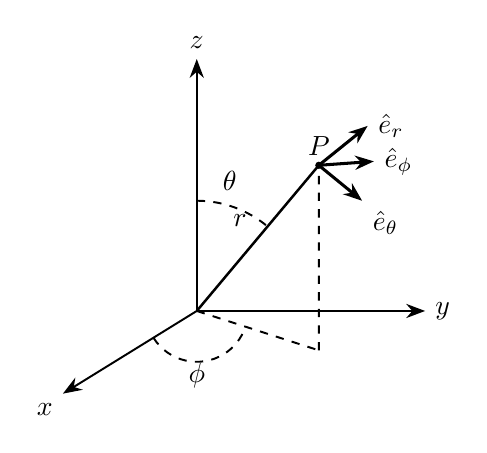
\begin{tikzpicture}[>={Stealth[length=2.4mm]}, line width=0.7pt]
  \coordinate (O) at (0,0);
  \draw[->] (O)--(-1.7,-1.05) node[below left]{$x$};
  \draw[->] (O)--(2.9,0) node[right]{$y$};
  \draw[->] (O)--(0,3.2) node[above]{$z$};
  \coordinate (F) at (1.55,-0.5);    % pie de P en xy
  \coordinate (P) at (1.55,1.85);
  \draw[dashed] (O)--(F) (F)--(P);
  \draw[line width=0.9pt] (O)--(P);  % r
  \fill (P) circle (1.3pt) node[above]{$P$};
  \node at (0.55,1.15){$r$};
  % theta (desde el eje z hacia r)
  \draw[dashed] (0,1.4) arc (90:50:1.4);
  \node at (0.42,1.65){$\theta$};
  % phi (en el plano xy)
  \draw[dashed] (-0.55,-0.34) arc (212:341:0.65);
  \node at (0.0,-0.82){$\phi$};
  % base en P
  \draw[->, line width=1.1pt] (P)--($(P)+(0.62,0.5)$) node[right]{$\hat e_r$};
  \draw[->, line width=1.1pt] (P)--($(P)+(0.55,-0.45)$) node[below right]{$\hat e_\theta$};
  \draw[->, line width=1.1pt] (P)--($(P)+(0.7,0.05)$) node[right]{$\hat e_\phi$};
\end{tikzpicture}
\end{document}
